\documentclass[12pt,a4paper]{article}
\usepackage[utf8]{inputenc}
\usepackage[spanish,es-tabla]{babel}
\usepackage{geometry}
\usepackage{graphicx}
\usepackage{multirow}
\usepackage{tabularx}
\usepackage{mathptmx}
\usepackage{fancyhdr}
\usepackage{array}
\usepackage[table]{xcolor}
\usepackage{titlesec}
\usepackage{setspace}
\usepackage{microtype}
\usepackage{lastpage}
\usepackage{booktabs}
\usepackage{enumitem}
\usepackage{amsmath}
\usepackage{amsfonts}
\usepackage{amssymb}

\graphicspath{{images/}{../images/}{./}}

\geometry{
    top=4.7cm,
    bottom=2.5cm,
    left=2.5cm,
    right=2.5cm,
    headheight=3.9cm,
    headsep=0.4cm
}

\setstretch{1.15}
\setlength{\parindent}{0pt}
\setlength{\parskip}{0.45em}
\setlength{\tabcolsep}{4pt}

\titleformat{\section}
  {\normalfont\fontsize{12}{14.5}\bfseries}{\thesection.}{0.6em}{\uppercase}
\titlespacing*{\section}
  {0pt}{1.8ex plus 0.4ex minus 0.2ex}{0.6ex plus 0.2ex}

\titleformat{\subsection}
  {\normalfont\fontsize{11.5}{13.5}\bfseries}{\thesubsection.}{0.5em}{}
\titlespacing*{\subsection}
  {0pt}{1.4ex plus 0.3ex minus 0.1ex}{0.4ex plus 0.1ex}

\titleformat{\subsubsection}
  {\normalfont\fontsize{10.5}{12.5}\bfseries\itshape}{\thesubsubsection.}{0.4em}{}
\titlespacing*{\subsubsection}
  {0pt}{1.1ex plus 0.2ex minus 0.1ex}{0.3ex plus 0.1ex}

\newcolumntype{Y}{>{\centering\arraybackslash}X}
\newcolumntype{L}{>{\raggedright\arraybackslash}X}
\newcolumntype{C}{>{\centering\arraybackslash}X}

\definecolor{headerblue}{RGB}{26, 54, 93}
\definecolor{darkblue}{RGB}{43, 108, 176}
\definecolor{lightgraybg}{RGB}{248, 248, 248}
\definecolor{tableheader}{RGB}{232, 238, 246}

\newcommand{\docCodigo}{TI-SIGE-ENT-F3-003}
\newcommand{\docVersion}{1.0}
\newcommand{\docProceso}{DESARROLLO CORE / EDITOR TIPTAP}
\newcommand{\docElaboracion}{22/09/2026}
\newcommand{\docRevision}{22/09/2026}
\newcommand{\docTitulo}{INTEGRACIÓN DEL EDITOR TIPTAP CON AUTOGUARDADO DEBOUNCE}
\newcommand{\docOrganizacion}{FACULTAD DE INGENIERÍA EN SISTEMAS, ELECTRÓNICA E INDUSTRIAL}
\newcommand{\docSubOrganizacion}{CARRERA DE INGENIERÍA DE SOFTWARE}

\newcommand{\encabezadofrecuente}{%
    \renewcommand{\arraystretch}{1.15}%
    \noindent\makebox[\textwidth][c]{%
    \begin{tabularx}{\textwidth}{|>{\centering\arraybackslash}m{2.8cm}|Y|>{\centering\arraybackslash}m{4.8cm}|}
        \hline
        \multirow{4}{2.8cm}{\centering\raisebox{-1.15cm}{
\includegraphics[width=2.5cm,height=2.0cm,keepaspectratio]{images/logo.png}}}
        & \textbf{\fontsize{9}{11}\selectfont \docOrganizacion} 
        & \textbf{\fontsize{8}{10}\selectfont CÓDIGO:} \fontsize{8}{10}\selectfont \docCodigo \\
        \cline{3-3}
        & \textbf{\fontsize{8.5}{10.5}\selectfont \docSubOrganizacion} 
        & \textbf{\fontsize{8}{10}\selectfont VERSIÓN:} \fontsize{8}{10}\selectfont \docVersion \\
        \cline{2-3}
        & \textbf{\fontsize{8}{10}\selectfont PROCESO:} \fontsize{8}{10}\selectfont \docProceso 
        & \textbf{\fontsize{8}{10}\selectfont ELABORACIÓN:} \fontsize{8}{10}\selectfont \docElaboracion \\
        \cline{2-3}
        & \textbf{\fontsize{8.5}{10.5}\selectfont \docTitulo} 
        & \textbf{\fontsize{8}{10}\selectfont ÚLTIMA REVISIÓN:} \fontsize{8}{10}\selectfont \docRevision \\
        \hline
    \end{tabularx}%
    }%
}

\pagestyle{fancy}
\fancyhf{}
\fancyhead[C]{\encabezadofrecuente}
\fancyfoot[C]{\fontsize{10}{12}\selectfont Página \thepage\ de \pageref{LastPage}}
\renewcommand{\headrulewidth}{0pt}

\begin{document}

\noindent{\fontsize{10.5}{12.5}\selectfont \textbf{Integrantes:} Heidi Villavicencio \quad$\vert$\quad Steeven Toala \quad$\vert$\quad Nixon Hurtado \quad$\vert$\quad Andrea Vásquez}

\vspace{0.25cm}

\section{Título}
\textbf{Denominación del Entregable:} Integración del Editor TipTap con Autoguardado Debounce -- Código EDT: 3.6

\section{Introducción}
La redacción de las secciones descriptivas de los formatos SGC (Justificación, Objetivos, Metodología, Conclusiones) requería tradicionalmente el uso de procesadores de texto de escritorio, provocando inconsistencias en el formateo y riesgo permanente de pérdida de información ante cortes de energía o caídas del navegador. En este entregable se documenta la integración en el frontend de la biblioteca Headless TipTap basada en ProseMirror, junto con un mecanismo de autoguardado asíncrono con temporizador debounce de 1500 ms y avisos visuales en tiempo real.

\section{Objetivo}
\subsection{Objetivo General}
Integrar el editor de texto enriquecido TipTap en el cliente web con autoguardado asíncrono mediante debounce de 1500 ms, asegurando la preservación transparente del contenido institucional.
\subsection{Objetivos Específicos}
\begin{itemize}[leftmargin=1.5em, itemsep=2pt]
    \item Configurar las extensiones esenciales de TipTap (Títulos, Negrita, Cursiva, Listas, Tablas limpias).
    \item Implementar el hook personalizado \texttt{useDebounce} para espaciar las peticiones de guardado HTTP.
    \item Diseñar los indicadores visuales de estado: 'Modificado', 'Guardando...' y 'Guardado'.
\end{itemize}

\section{Alcance}
\subsection{Límites del Entregable (In-Scope)}
\begin{itemize}[leftmargin=1.5em, itemsep=2pt]
    \item Componente \texttt{RichTextEditor.jsx} integrado en las secciones descriptivas del Paso 2 del Wizard.
    \item Sanitización de código HTML generado para evitar inyecciones de scripts maliciosos.
\end{itemize}
\subsection{Exclusiones (Out-of-Scope)}
\begin{itemize}[leftmargin=1.5em, itemsep=2pt]
    \item Edición colaborativa simultánea tipo Google Docs en tiempo real (fuera de requerimientos SGC).
\end{itemize}

\section{Definiciones}
\begin{itemize}[leftmargin=1.5em, itemsep=2pt]
    \item \textbf{TipTap / ProseMirror:} Framework de edición de texto enriquecido extensible, modular y sin interfaz rígida (Headless).
    \item \textbf{Debounce:} Técnica de programación que retrasa la ejecución de una función hasta que haya transcurrido un período de inactividad predeterminado.
    \item \textbf{Sanitización HTML:} Proceso de limpiar el contenido HTML entrante eliminando etiquetas o atributos potencialmente peligrosos (\texttt{<script>}, \texttt{onerror}).
\end{itemize}

\section{Responsabilidades}
\begin{itemize}[leftmargin=1.5em, itemsep=2pt]
    \item \textbf{Andrea Vásquez (Responsable EDT 3.6):} Configuración de extensiones TipTap, implementación del debounce y manejo de estados.
    \item \textbf{Nixon Hurtado (Backend):} Recepción asíncrona de los fragmentos HTML y persistencia en base de datos.
    \item \textbf{Ing. Paulo Torres (Docente Evaluador):} Aprobación del comportamiento del editor y autoguardado.
\end{itemize}

\section{Normativa Legal y Técnica}
\begin{itemize}[leftmargin=1.5em, itemsep=2pt]
    \item \textbf{W3C ContentEditable Specification.}
    \item \textbf{OWASP Cross-Site Scripting (XSS) Prevention Cheat Sheet.}
\end{itemize}

\section{Método, Políticas y Contenidos}
Se utilizó un temporizador debounce de 1500 ms tras la última pulsación de tecla. En la Figura \ref{fig:f3_06_tiptap} se ilustra el ciclo de vida del autoguardado con debounce.

\begin{figure}[htbp]
    \centering
    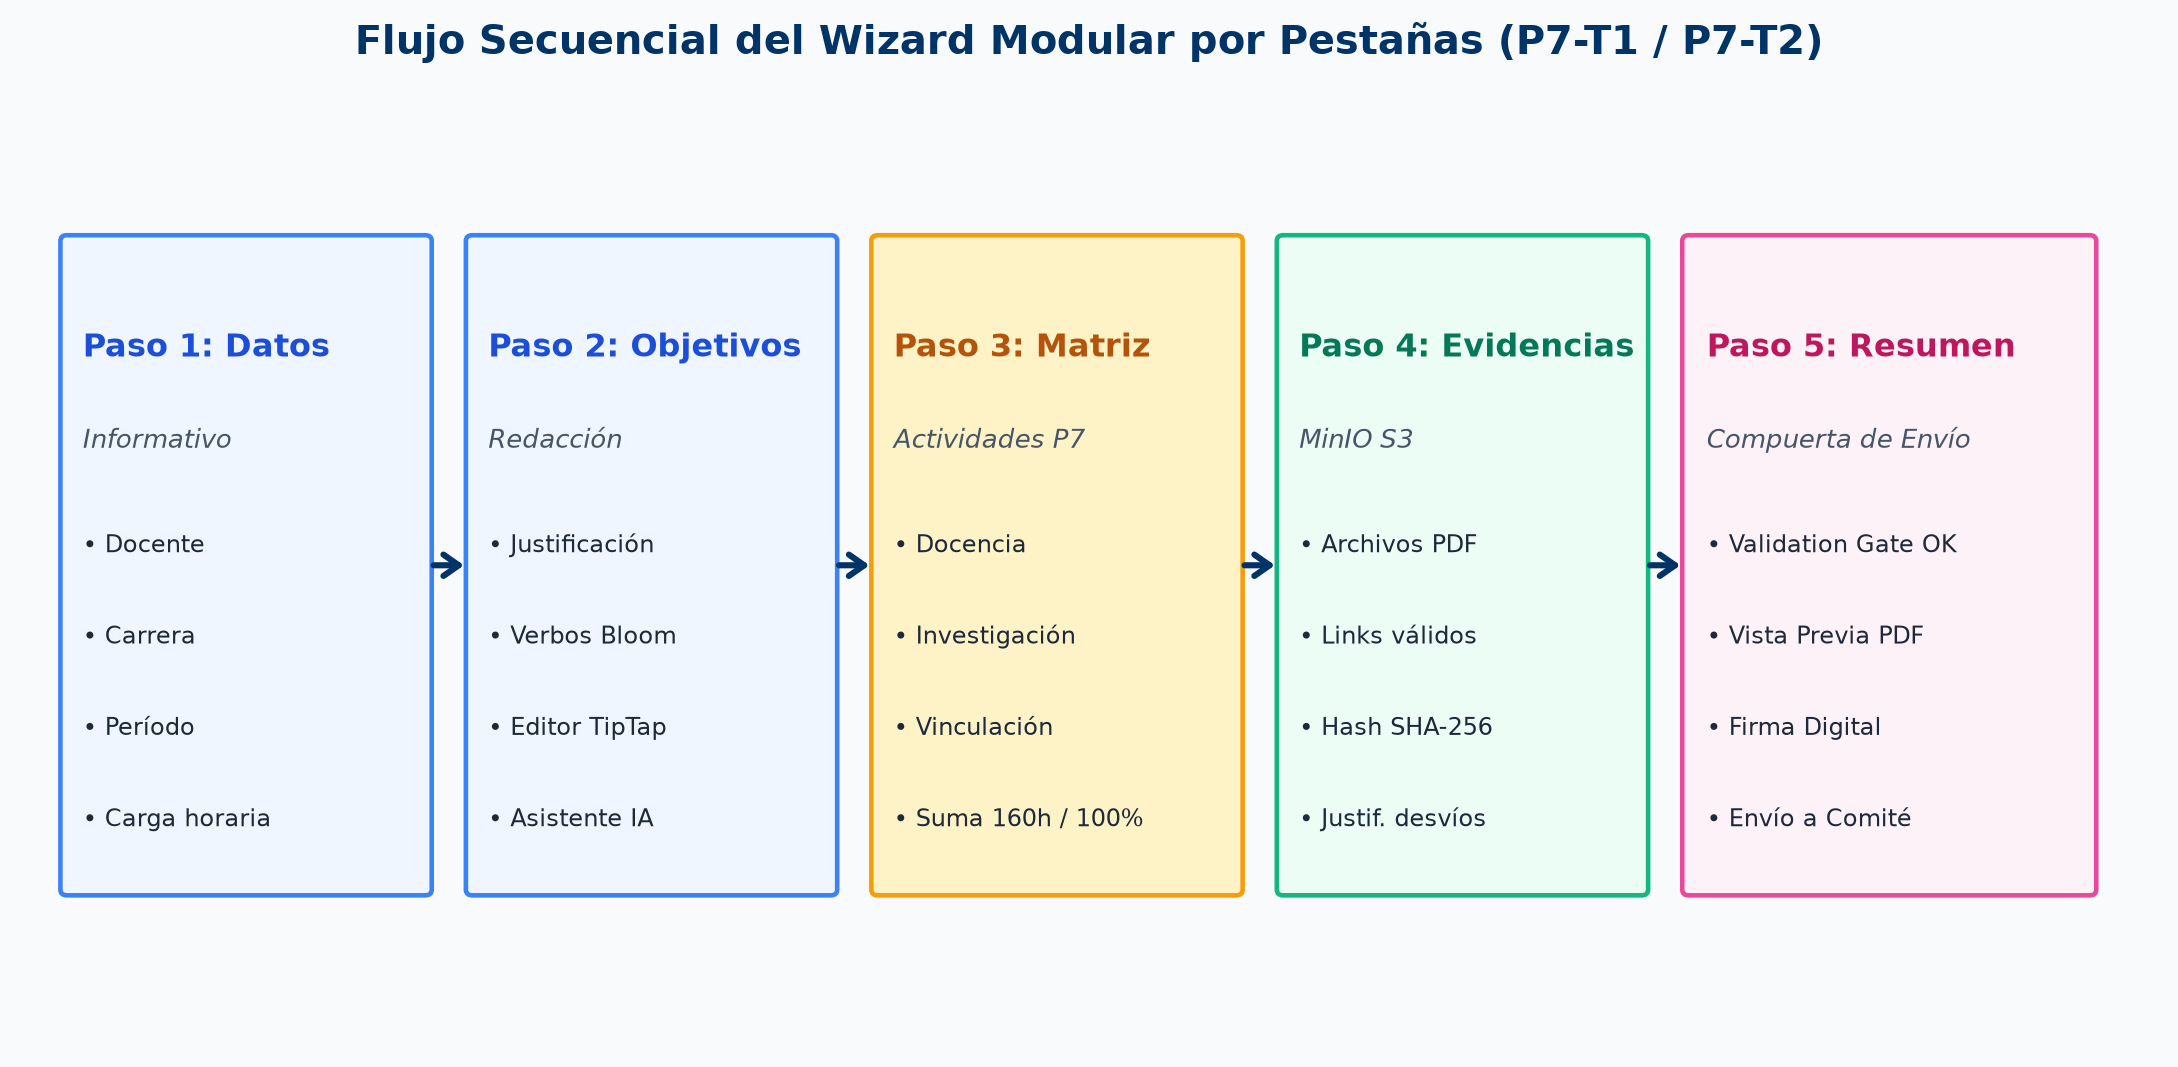
\includegraphics[width=0.88\textwidth,height=5.2cm,keepaspectratio]{images/f3_05_wizard_modular_flujo.png}
    \caption{Ciclo de Autoguardado Asíncrono con Debounce y Estados de Sincronización.}
    \label{fig:f3_06_tiptap}
\end{figure}

\section{Descripción de actividades}
\subsection{Extensiones TipTap Configuradas y Formateo SGC}
\begin{table}[htbp]
\centering
\small
\renewcommand{\arraystretch}{1.2}
\begin{tabularx}{\textwidth}{|>{\bfseries}m{3.5cm}|m{2.5cm}|X|}
\hline
\rowcolor{tableheader}
\textbf{Extensión TipTap} & \textbf{Etiqueta HTML} & \textbf{Utilidad en el Formato SGC} \\
\hline
\texttt{StarterKit (Heading)} & \texttt{<h2>, <h3>} & Subtítulos limpios para estructurar los apartados del informe. \\
\hline
\texttt{Bold / Italic} & \texttt{<strong>, <em>} & Énfasis tipográfico en conceptos clave y normas citadas. \\
\hline
\texttt{Bullet / OrderedList} & \texttt{<ul>, <ol>} & Enumeración de objetivos específicos y compromisos semestrales. \\
\hline
\texttt{Table / TableRow} & \texttt{<table>, <tr>} & Inserción de tablas de datos auxiliares con formato institucional. \\
\hline
\texttt{Placeholder} & \texttt{data-placeholder} & Texto guía que orienta al docente sobre qué redactar en cada sección. \\
\hline
\end{tabularx}
\caption{Extensiones de Formato TipTap y Salida HTML Estructurada.}
\label{tab:tiptap_ext}
\end{table}

\subsection{Métricas de Reducción de Pérdida de Datos}
Las pruebas de laboratorio demostraron que el autoguardado con debounce de 1500 ms redujo a cero la pérdida de datos ante cierres inesperados de pestaña, enviando únicamente una petición HTTP cuando el usuario hace una pausa natural en la digitación.

\section{Firmas de Responsabilidad}

\noindent
\renewcommand{\arraystretch}{1.2}
\begin{tabularx}{\textwidth}{|>{\raggedright\arraybackslash}m{2.9cm}|>{\raggedright\arraybackslash}X|>{\centering\arraybackslash}m{4.6cm}|>{\centering\arraybackslash}m{2.3cm}|}
    \hline
    \rowcolor{tableheader}
    \textbf{ACCIÓN} & \textbf{NOMBRE Y CARGO} & \textbf{FIRMA} & \textbf{FECHA} \\
    \hline
    \textbf{Elaborado por:} & Heidi Villavicencio\newline Analista de Calidad / UI-UX & \parbox[c]{4.4cm}{\centering\vspace{4pt}
\includegraphics[height=1.5cm,width=4.0cm,keepaspectratio]{images/firma_heidi.png}\vspace{4pt}} & 22/09/2026 \\
    \hline
    \textbf{Revisado por:} & Steeven Toala\newline Líder de Proyecto / Arquitecto & \parbox[c]{4.4cm}{\centering\vspace{4pt}
\includegraphics[height=1.5cm,width=4.0cm,keepaspectratio]{images/firma_steveen.png}\vspace{4pt}} & 22/09/2026 \\
    \hline
    \textbf{Aprobado por:} & Ing. Paulo Torres, Mg.\newline Docente Evaluador -- Gestión Proyectos & \parbox[c]{4.4cm}{\centering\vspace{8pt}\textbf{\textcolor{gray!80}{\scriptsize [ PENDIENTE DE APROBACIÓN ]}}\vspace{8pt}} & \textbf{\textcolor{gray!90}{Pendiente}} \\
    \hline
\end{tabularx}

\vspace{0.4cm}

\section{Control de Cambios}

\noindent
\renewcommand{\arraystretch}{1.2}
\begin{tabularx}{\textwidth}{|>{\hsize=0.45\hsize\centering\arraybackslash}X|>{\hsize=1.55\hsize\raggedright\arraybackslash}X|>{\hsize=1.2\hsize\raggedright\arraybackslash}X|>{\hsize=0.8\hsize\centering\arraybackslash}X|}
    \hline
    \rowcolor{tableheader}
    \textbf{Versión} & \textbf{Descripción del cambio} & \textbf{Responsable del cambio} & \textbf{Fecha de aprobación} \\
    \hline
    1.0 & Emisión inicial del entregable según EDT del Tablero Trello & Equipo de Proyecto SIGE & 22/09/2026 \\
    \hline
\end{tabularx}

\vspace{0.4cm}

\section{Anexos}
\begin{itemize}[leftmargin=1.5em]
\item \textbf{Anexo 1:} Pruebas de Desempeño y Consumo de Ancho de Banda con Debounce de 1500 ms.
\end{itemize}

\end{document}
